\documentclass{beamer}

% theme
\usetheme{Darmstadt}

% packages
\usepackage{mathtools}
\usepackage[]{hyperref}
\usepackage{xcolor}
\usepackage{verbatimbox}
\usepackage{subcaption}

% hyperref setup
\hypersetup{colorlinks, linkcolor=, urlcolor=blue}

% custom definitions
\def\Cplusplus{{C\raise.2ex\hbox{++}}}
\definecolor{light-gray}{gray}{0.85}

\begin{document}
\title{ChemTools} 
\author{Ahmad El Sayed} 
\date{\today} 

\begin{frame}
  \titlepage
\end{frame}

\begin{frame}
\frametitle{Table of contents}
\tableofcontents
\end{frame}

\section{Introduction} 
\subsection{ChemTools}
\begin{frame}
\frametitle{What is ChemTools?}
\begin{itemize}
  \item ChemTools is a collection of thermochemical tools
  \item Available on \href{https://github.com/ahmades/ChemTools}{GitHub} under the MIT license
  \item Language: \Cplusplus
  \item Build system: CMake
  \item Catch2 Unit tests
\end{itemize} 
\end{frame}

\subsection{Features}
\begin{frame}
\frametitle{Completed and planned features}
\begin{itemize}
  \item Closed homogeneous chemical reactors with one or two properties held constant:
  \begin{itemize}
    \item pressure,
    \item volume,
    \item temperature and pressure, or
    \item temperature and volume.
  \end{itemize} 
  \item \textcolor{light-gray}{Closed homogeneous chemical reactors with user-defined Python scripts providing functions for:}
  \begin{itemize}
    \item \textcolor{light-gray}{the volume and its time derivative as a function of time, or}
    \item \textcolor{light-gray}{the temperature and pressure as a function of time.}
  \end{itemize}
  \item \textcolor{light-gray}{Flamelet library generator base:}
  \begin{itemize}
    \item \textcolor{light-gray}{the $\beta$-PDF approach, or}
    \item \textcolor{light-gray}{the Presumed Mapping Function approach}.
  \end{itemize}
\end{itemize} 
\end{frame}

\section{Chemical reactors}
\subsection{Concepts}
\begin{frame}
\frametitle{What is a closed homogeneous reactor?}
\begin{itemize}
  \item An enclosed volume in which a chemical reaction takes place, i.e. a chemical process vessel
  \item No inlets or outlets
  \item An initial gas mixture exists at an given initial state:
  \begin{itemize}
   \item Species composition
   \item Pressure
   \item Temperature
   \item Volume  
  \end{itemize}
  \item The gas mixture reacts from this initial state over a specified period of time
  \item Purpose: used to understand chemical processes through reaction kinetics
\end{itemize} 
\end{frame}

\subsection{Physical and mathematical model}
\begin{frame}
\frametitle{Governing equations of closed homogeneous reactors}
\begin{footnotesize}
\begin{itemize}
  \item Zero dimensional reactors: transient and space-independent
  \item Mass and energy conservation in a mixture containing $K$ species:
  \begin{equation*}
    \text{IVP ODE system }
    \begin{dcases}
      \textcolor{magenta}{\rho} \frac{d\textcolor{red}{Y_k}}{d\textcolor{green}{t}} = 
      \textcolor{cyan}{W_k} \textcolor{blue}{\dot\omega_k}, \quad k = 1,2, \ldots, K \\
      \textcolor{magenta}{\rho} \textcolor{orange}{c_p} \frac{d\textcolor{red}{T}}{dt} = 
      \sum_{k=1}^K h_k \textcolor{cyan}{W_k} \textcolor{blue}{\dot\omega_k}
    \end{dcases}
  \end{equation*}
  \begin{equation*}
    \begin{aligned}
      &\textcolor{red}{Y_k} = \text{ mass fraction of species } k \text{ (dependent variables)}\\
      &\textcolor{red}{T} = \text{ temperature (dependent variables)}\\
      &\textcolor{green}{t} = \text{ time (independent variable)}\\
      &\textcolor{blue}{\dot\omega_k = \dot\omega_k(Y_1,Y2, \ldots, Y_K, T)} 
       = \text{ net chemical production rate (non-linear)}\\
      &\textcolor{magenta}{\rho} = \text{density} \\
      &\textcolor{cyan}{W_k} =\text{molecular weight of species } k\\
      &h_k =\text{specific enthalpy of species } k\\
      &\textcolor{orange}{c_p} =\text{specific heat at constant pressure}
    \end{aligned}
  \end{equation*}
  \item Fast and slow time scales lead to a stiff ODE system
\end{itemize}
\end{footnotesize}
\end{frame}

\section{Description}
\subsection{Project description}
\begin{frame}
\frametitle{Description and dependencies}
\begin{figure}
  \centering
  \includegraphics[width=0.8\linewidth]{figures/svg/ChemTools.png}
\end{figure}
\begin{tiny}
Other libraries:
\begin{itemize}
  \item \href{https://github.com/LLNL/units}{LLNL} units for the handling of physical units
  \item \href{https://github.com/fmtlib/fmt}{fmt} for formatting
  \item Python C API
  \item Various Boost libraries: filesystem, optional, algorithm, etc.
  \item \href{https://github.com/gabime/spdlog}{spdlog} for logging (coming soon)
  \item \href{https://gitlab.com/libeigen/eigen}{Eigen} for numerical linear algebra
\end{itemize}
\end{tiny}
\end{frame}

\subsection{Input}
\begin{frame}[fragile]\frametitle{YAML input configuration}
\vspace{-0.35cm}
\begin{minipage}{.3\textwidth}
 \begin{figure}
  \centering
  \includegraphics[width=0.5\linewidth]{figures/yaml.png}
\end{figure}
\end{minipage}
\begin{minipage}{.6\textwidth}
\begin{verbnobox}[\fontsize{6pt}{6pt}\selectfont]
- Reactor:        CONSTANT_PRESSURE
  Mechanism:
    Description:  Constant pressure reactor 1
    Path:         ../data/gri30.cti
  Description:    case set 1
  Cases:
    Case:
      Description: useful case 1.1
      Pressure:
        Unit:  Pa
        Value: 101325.0
      Temperature:
        Unit:  Kelvin
        Value: 1300.0
      Composition:
        Type:  mole fraction
        Value: [[CH4, 0.1], [O2, 0.5], [N2, 0.4]]
      Time:
        Unit:  ms
        Value: 1.0
    Case:
      Description: useful case 1.2
      Pressure:
        Unit:  atm
        Value: 2.0
      Temperature:
        Unit:  degC
        Value: 25.0
      Composition:
        Type:  concentration
        Unit:  kmol/cm^3
        Value: [[CH4, 0.1], [O2, 0.5], [N2, 0.4]]
      Time:
        Unit:  min
        Value: 1.0
\end{verbnobox}
\end{minipage}
\end{frame}

\subsection{Output}
\begin{frame}
\frametitle{HDF5 output}
\begin{figure}
\centering
\begin{subfigure}{.12\textwidth}
  \centering
  \includegraphics[width=\linewidth]{figures/hdf.png}
\end{subfigure}
\begin{subfigure}{.84\textwidth}
  \centering
  \includegraphics[width=\linewidth]{figures/output.png}
\end{subfigure}
\end{figure}
\end{frame}

\subsection{Structure}
\begin{frame}
\frametitle{Project structure and general implementation details}
\vskip-0.35cm
\begin{figure}
  \centering
  \includegraphics[width=0.63\linewidth]{figures/svg/project_tree.png}
\end{figure}
\end{frame}

\section{Demo}
\subsection{Closed reactor demo}
\begin{frame}[fragile]\frametitle{Constant volume reactor: hydrogen oxidation}
\begin{tiny}
  \begin{itemize}
    \item Hydrogen oxidation at constant volume
    \item Global reaction: $2H_2 + O_2 \rightarrow 2H_2O + \text{ Heat}$ (not realistic)
    \item Many more intermediate species: $OH, O, H, H_2O_2, HO_2$, etc.
  \end{itemize}
\end{tiny}
\begin{minipage}{.3\textwidth}
\begin{verbnobox}[\fontsize{4pt}{4pt}\selectfont]
- Reactor: CONSTANT_VOLUME
  Mechanism:
    Description: GRI-Mech 3.0
    Path: ../data/gri30.cti
  Description: case set 1
  Cases:
    Case:
      Description: Combustion of hydrogen
      Pressure:
        Unit:  atm
        Value: 1.0
      Temperature:
        Unit:  Kelvin
        Value: 1001.0
      Composition:
        Type:  mole fraction
        Value: [[CH4,2.0], [O2,1.0], [N2,4.0]]
      Time:
        Unit:  ms
        Value: 1.0
\end{verbnobox}
\end{minipage}
\hspace{0.1cm}
\begin{minipage}{.55\textwidth}
\begin{figure}
  \centering
  \includegraphics[width=0.99\linewidth]{figures/results/results.png}
\end{figure}
\end{minipage}
\end{frame}

\section*{}
\begin{frame}
\begin{center}
 \Huge Thank you
\end{center}
\end{frame}

\end{document}

